% N.B. one {latexonly} environment commented out so that its
% contents can be displayed in the HTML version of this template.
% Uncomment it for actual use!
%
% Use text editor to replace:
%
%       author   --- author's login name
%       thisdoc  --- document filename (as in thisdoc.tex, thisdoc.ps)
%       psiz     --- size of compressed PostScript file
%
%       Document_Date          --- current date
%       Document_Short_Title   --- header text for Postscript
%       Document_Long_Title    --- full document title
%       Author_Name            --- full author name
%       Author_City            --- Charlottesville, Socorro, etc.
%       Author_State           --- Virginia, New Mexico, etc.
%
%       (non-NRAO: also replace institute name/acronym and country?)
%

\documentclass{article}
\usepackage{html,makeidx,epsf}
\usepackage{graphicx}
\renewcommand{\bibname}{References}

%
% Add home page navigation button -- edit the URL!
%


\htmladdtonavigation{\htmladdnormallink
  {\htmladdimg{../jetscalecropped.png}}{https://www.dropbox.com/s/jem3l3jabcyex9s/Curriculum_Vitae_Ilari_Angervuori.pdf?dl=0}}

%
% define hyperlink URLs:
%

\def\linkedin{https://www.linkedin.com/in/ilari-angervuori-0a1358160/}
\def\soundcloud{https://soundcloud.com/ilari-angervuori}
\def\github{https://github.com/Rugiero}
\def\cv{}
\makeindex

\begin{document}

%
%  Page formatting for Postscript output
%

\title{
{\bf A glimpse to my mind}
}

\author
{
Ilari Angervuori\\
}

\date
{
{Updated 11.02.2021}\\
}

\begin{center}
  \htmladdnormallink{Linkedin}{\linkedin}\\
  \htmladdnormallink{Soundcloud}{\soundcloud}\\
  \htmladdnormallink{GitHub}{\github} \\
  \htmladdnormallink{CV}{\cv}
\end{center}

%\begin{latexonly}
\markright{Document_Short_Title}
\maketitle
% uncomment to run:
%\end{latexonly}

\tableofcontents

\pagebreak
\chapter{About me}
I am a mathematician and engineer from Finland. You can find about my professional achievements below.

I am keeping up a monthly blog what you can find in the blog posts section. It handles daily stuff encountered in my professional life sometimes with a poetic undertone (first thing taught to a fresh PhD student: ``Don't try to be poetic''). I hope you will find it interesting. 

In free time I love music, literature, long walks, coffee and beer.


\begin{figure}
  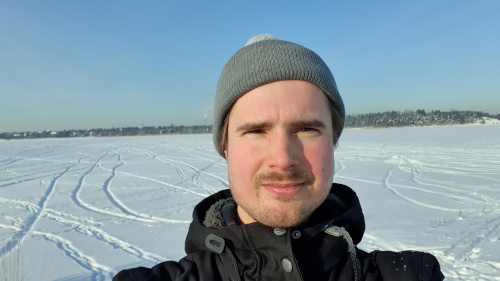
\includegraphics[width=\linewidth]{me1.jpg}
  \caption{Me in my beloved home town Helsinki (well, technically in Espoo, Otaniemi)}
\end{figure}

\section{Education}
\begin{itemize}
\item 2016 Bachelor of Science University of Helsinki\\
\item 2018 Master of Philosophy University of Helsinki
\end{itemize}
\section{Research}

\begin{itemize}
\item Downlink Coverage and Rate Analysis of Low Earth Orbit Satellite Constellations Using Stochastic Geometry
Okati, N., Riihonen, T., Korpi, D., Angervuori, I. & Wichman, R., Aug 2020, In : IEEE Transactions on Communications. 68, 8, p. 5120-5134 9079921.\\
\end{itemize}


\chapter{Blog posts}
General thoughts on mathematics and engineering, practical instructions, artistic non sense. The themes of this blog are much inspired by challenges encountered in my professional life.

\section{2021}
Hope it will be better than $2020.$
\subsection{February}
\subsubsection{Controlling your passwords with pass}
Pass is a nice unix style free and open source wallet for keeping your passwords safe. Here is a brief look how to set it up in Ubuntu.

\begin{itemize}
\item Install the application in the terminal \\
\begin{verbatim}
sudo apt install pass  
\end{verbatim}
\item Check for existing GPG keys \\
\label{1}
\begin{verbatim}
gpg --list-keys 
\end{verbatim}
\item If no keys were found generate a key pair \\
\begin{verbatim}
gpg --generate-key
\end{verbatim}
\item Copy the name of the key and initalize pass\\
\begin{verbatim}
pass init ABCDEFGHIJKLMNOPQRSTUV1234, 
\end{verbatim}
where ABCDEFGHIJKLMNOPQRSTUV1234 is the name of the key.
\item Generate a password with \\
\begin{verbatim}
pass generate keyfolder/newkey 
\end{verbatim}
List passwords
\begin{verbatim}
pass
\end{verbatim}
Copy a password to clipboard \\
\begin{verbatim}
pass keyfolder/newkey -c
\end{verbatim}
For more commands
\begin{verbatim}
man pass
\end{verbatim}
\end{itemize}

Connect pass to git so it is easy to keep track of changes with multiple machines.

\begin{itemize}
\item Export your public and private key to a file with \\
  \begin{verbatim}
gpg --export --output public.key ABCDEFGHIJKLMNOPQRSTUV1234 
gpg --export-secret-key --output private.key ABCDEFGHIJKLMNOPQRSTUV1234,
  \end{verbatim}
  where ABCDEFGHIJKLMNOPQRSTUV1234 is your keyname.\\
\item Now we can initilize the git reporisoritory with these keys. Move public.key and private.key through a safe channel to a computer you wish to use pass in. Import the keys to the machine \\
\begin{verbatim}
gpg --import public.key
gpg --import private.key
\end{verbatim}
\item After importing keys to a new machine you can initilize pass
\begin{verbatim}
pass init ABCDEFGHIJKLMNOPQRSTUV1234
\end{verbatim}

\item Initalize your git repository. Make a new repository named pass-store e.g. to GitHub if you are doing this first time before the following commands\\
\begin{verbatim}
pass git init 
pass git remote add origin git@repo.com:myname/pass-store
 \end{verbatim}
\item Get password data from the server (from a non-empty repository, otherwise skip)
\begin{verbatim}
pass git pull origin master --allow-unrelated-histories
\end{verbatim}
\item Do some changes and pass will automatically commit them. Push and set upstream \\
\begin{verbatim}
pass git push --set-upstream origin master 
\end{verbatim}
\item From here on you can use the familiar git commands \\
\begin{verbatim}
pass git pull 
pass git push 
\end{verbatim}
\end{itemize}
Stay safe :)

\vspace{2cm}
References:
  \bibitem{stochasticgeometry}
    https://www.passwordstore.org/



%
% optional post-title formatting for PostScript
%
\parindent0pt
\parskip2.5ex plus 0.5ex minus 0.5ex
